\PassOptionsToPackage{unicode=true}{hyperref} % options for packages loaded elsewhere
\PassOptionsToPackage{hyphens}{url}
%
\documentclass[]{article}
\usepackage{lmodern}
\usepackage{amssymb,amsmath}
\usepackage{ifxetex,ifluatex}
\usepackage{fixltx2e} % provides \textsubscript
\ifnum 0\ifxetex 1\fi\ifluatex 1\fi=0 % if pdftex
  \usepackage[T1]{fontenc}
  \usepackage[utf8]{inputenc}
  \usepackage{textcomp} % provides euro and other symbols
\else % if luatex or xelatex
  \usepackage{unicode-math}
  \defaultfontfeatures{Ligatures=TeX,Scale=MatchLowercase}
\fi
% use upquote if available, for straight quotes in verbatim environments
\IfFileExists{upquote.sty}{\usepackage{upquote}}{}
% use microtype if available
\IfFileExists{microtype.sty}{%
\usepackage[]{microtype}
\UseMicrotypeSet[protrusion]{basicmath} % disable protrusion for tt fonts
}{}
\IfFileExists{parskip.sty}{%
\usepackage{parskip}
}{% else
\setlength{\parindent}{0pt}
\setlength{\parskip}{6pt plus 2pt minus 1pt}
}
\usepackage{hyperref}
\hypersetup{
            pdfborder={0 0 0},
            breaklinks=true}
\urlstyle{same}  % don't use monospace font for urls
\usepackage[margin=1.0in]{geometry}
\usepackage{graphicx,grffile}
\makeatletter
\def\maxwidth{\ifdim\Gin@nat@width>\linewidth\linewidth\else\Gin@nat@width\fi}
\def\maxheight{\ifdim\Gin@nat@height>\textheight\textheight\else\Gin@nat@height\fi}
\makeatother
% Scale images if necessary, so that they will not overflow the page
% margins by default, and it is still possible to overwrite the defaults
% using explicit options in \includegraphics[width, height, ...]{}
\setkeys{Gin}{width=\maxwidth,height=\maxheight,keepaspectratio}
\setlength{\emergencystretch}{3em}  % prevent overfull lines
\providecommand{\tightlist}{%
  \setlength{\itemsep}{0pt}\setlength{\parskip}{0pt}}
\setcounter{secnumdepth}{0}
% Redefines (sub)paragraphs to behave more like sections
\ifx\paragraph\undefined\else
\let\oldparagraph\paragraph
\renewcommand{\paragraph}[1]{\oldparagraph{#1}\mbox{}}
\fi
\ifx\subparagraph\undefined\else
\let\oldsubparagraph\subparagraph
\renewcommand{\subparagraph}[1]{\oldsubparagraph{#1}\mbox{}}
\fi

% set default figure placement to htbp
\makeatletter
\def\fps@figure{htbp}
\makeatother

\usepackage{palatino}
\usepackage{setspace}
\doublespacing
\usepackage[left]{lineno}
\linenumbers

\author{}
\date{\vspace{-2.5em}}

\begin{document}

\hypertarget{environmental-and-genetic-contributions-to-ecogeographic-rules-in-house-mice}{%
\section{Environmental and genetic contributions to ecogeographic rules
in house
mice}\label{environmental-and-genetic-contributions-to-ecogeographic-rules-in-house-mice}}

\vspace{20mm}

Mallory A. Ballinger and Michael W. Nachman\({^\dagger}\)

\vspace{20mm}

Department of Integrative Biology

Museum of Vertebrate Zoology

University of California, Berkeley

Berkeley, CA 94702-3160

\vspace{10mm}

\({\dagger}\) To whom orrespondence should be addressed:

\href{mailto:mnachman@berkeley.edu}{mnachman@berkeley.edu}

\vspace{40mm}

\textbf{Running title:} Allen's rule and Bergmann's rule in house mice

\newpage

\hypertarget{abstract-200-words}{%
\subsection{Abstract (200 words)}\label{abstract-200-words}}

\newpage

\hypertarget{introduction}{%
\subsection{Introduction}\label{introduction}}

Clines in phentoypes have historically been attributed to natural
selection that reflect adaptation to local environments (Huxley 1938;
Endler 1977). Two of the most well described phenotypic clines are
Allen's rule and Bergmann's rule. Allen's rule (Allen 1877) predicts
that organisms have shorter appendages at higher latitudes than those
closer to the equator. Similarly, Bergmann's rule (Bergmann 1847)
proposes that organisms at higher latitudes are larger in size than
those closer to the equator. Although explanatations for these
ecogeographic rules continues to be debated (REFs), the overarching
hypothesis is that of heat conservation in colder climates by decreasing
surface area to volume ratios (REFs). Numerous studies have documented
Bergmann's rule and Allen's rule within and across species of mammals
(REFs), birds (REFs), and even in humans (REFs). Various meta-analyses
have also been conducted, either supporting (REFs) or refuting (REFs) an
evolutionary basis to these phenotypic clines. These contradicting
results are unsurprising, given the variation in datasets and choice of
environmental correlates used in each study. To date, we still have very
little understanding of the mechanisms underlying these broad phenotypic
clines.

Missing from these discussions are careful analyses determining which
traits are genetically encoded and/or environmentally influenced. Many
of the traits underlying Bergmann's rule and Allen's rule are
quantitative, thus they are polygenic and environmentally determined
(Harpak and Przeworski 2021). Dissentangling genetics from environmental
effects is impossible with phenotypic data collected on wild-caught
specimens. Clines in phenotypes may be masked in the wild by
environmental effects and possbile genotype-by-environment interactions
(REFs). Thus, cryptic variation in traits consistent with either
Bergmann's rule or Allen's rule can exist underneath environmental
effects, which are hidden in studies relying soley on wild-caught
phenotypic data. Moreover, less attention has been given to the
environmental influences of these traits (but see (James 1983)), likely
due to the difficulty in controlling for environmental effects via
transplant experiments or common garden experiments. These limitations
have impeded our ability to make substantial progress on understanding
the mechanisms behind Bergmann's rule and Allen's rule.

House mice (\emph{Mus musculus domesticus}) are a tractable system to
dissentangle genetics from environment underlying complex traits. House
mice are endemic to Western Europe, but through European colonization,
have expanded their range across broad latitudinal distributions of the
Americas. They can be found from the tip of South America up to Alaska,
spanning temperate and tropical environments (Phifer-Rixey and Nachman
2015), making them an ideal system to test for ecogeographic rules.
Although house mice have only resided in these novel environments for
\textasciitilde{}500 generations, there is evidence for clinal
adaptation across populations. Specifically, mice in eastern North
America follow Bergmann's rule (Lynch 1992), with larger mice in more
northern populations compared to their southern conspecifics. Moreover,
these body size differences persist in a commmon environment and over
many generations, indicating a genetic basis for Bergmann's rule in
house mice (Lynch 1992; Phifer-Rixey et al. 2018). Additionally, earlier
work in Australian house mice revealed an environmental influence on
tail length when exposed to cold temperatures (Barnett and Dickson
1984). Specficially, wild mice housed at cold temperatures grew
significantly shorter tails than mice reared at warm temperatures
(Barnett and Dickson 1984). However, this study only investigated a
single population of house mice, making it difficult to place these
results in an explicit evolutionary framework. Overall, we still know
very little regarding phenotpic variation of house mice across their
entire latitudinal distribution, and the subsequent contributions of
genetics and the enviornment on these complex traits.

Here, we use a combination of approaches to tease apart genetics from
plasticity in Bergmann's rule and Allen's rule in American house mice.
First, we determined if house mice conform to both Bergmann's rule and
Allen's rule across their entire introduced range by analyzing
phenotypic data from wild-caught individuals across North and South
America. Second, because it is difficult to dissentangle genetics from
plasticity using wild phenotypic data, we collected temperate and
tropical populations of house mice from the ends of their latitudinal
distribution, brought them back to the lab, and established wild-derived
colonies. We analyzed phenotypic differences between populations and
across generations in a common environment to identify a genetic basis
for Allen's rule and Bergmann's rule. Third, to measure the influence of
the environment on body size and extremity length, we performed a common
garden experiment by rearing both populations of house mice in warm and
cold temperatures and measuring the effects on body size and tail
length. Measuring developmental plasticity in these traits allows us to
assess the influence of developmental temperature on Bergmann's rule and
Allen's rule. Lastly, using classic reaction norm analyses, we show that
unlike body size, tail length is highly plastic and the plastic response
goes in the same direction as the evolved response, highlighting an
example of adaptive phentoypic plasticity.

\newpage

\hypertarget{materials-and-methods}{%
\subsection{Materials and Methods}\label{materials-and-methods}}

\hypertarget{wild-caught-phenotypic-metadata}{%
\subparagraph{\texorpdfstring{\emph{Wild-caught phenotypic
metadata}}{Wild-caught phenotypic metadata}}\label{wild-caught-phenotypic-metadata}}

Specimen data from wild house mice collected across several North and
South American latitudinal transects were downloaded from the
``Environmental adaptation in introduced populations of house mice, Mus
musculus, across the Americas'' project in Arctos
(\url{http://arctosdb.org}). Details regarding the collection of these
data have been previously described (Phifer-Rixey et al. 2018; Suzuki et
al. 2019\emph{a}, 2019\emph{b}, 2020). Briefly, house mice were
collected across two transects in North America in summer 2012
(Phifer-Rixey et al. 2018; Suzuki et al. 2020), and along two transects
in South America in 2013 and 2014 (Suzuki et al. 2019\emph{a}, 2020).
Mice were collected during the warmest months of the year for each
transect. Standard museum measurements were recorded for each mouse,
including sex, reproductive status, total body length, tail length, hind
foot length, ear length, and body weight. Pregnant females, juveniles,
subadults, and individuals collected over 1,500m in elevation were
removed from downstream analyses. Tail lengths that were shorter than
20mm were considered outliers and removed from downstream analyses.
Sample information for the Arctos dataset (n = 215) is provided in Table
SX.

To obtain a larger dataset of wild house mice, we obtained records of
all house mice collected across the Americas by downloading museum
specimens from VertNet (\url{http://vertnet.org}) in October of 2020,
using the search query: \emph{vntype}:specimen, \emph{genus}:Mus. We
filtered records to only include specimens that were collected in North
or South America (excluding islands). We removed all known pregnant
females, juveniles, and subadults. Sample information for the VertNet
dataset (n = 3,016) is provided in Table SXX.

\hypertarget{laboratory-reared-mice---common-garden-experiment-1}{%
\subparagraph{\texorpdfstring{\emph{Laboratory-reared mice - common
garden experiment
1}}{Laboratory-reared mice - common garden experiment 1}}\label{laboratory-reared-mice---common-garden-experiment-1}}

For the first common garden experiment, live animals were collected from
two locations that represent the ends of the house mouse latitudinal
distribution: Manaus, Amazonas, Brazil (MAN) and Saratoga Springs, New
York, USA (SAR). Details of this common garden experiment are specified
in (Phifer-Rixey et al. 2018; Suzuki et al. 2020). Briefly, live mice
from both Brazil and New York were brought back to the lab at the
University of California, Berkeley. Within each population, unrelated
pairs of wild-caught mice were mated to produce first generation (N1)
lab-reared mice, and these inbred lines have subsequently been
maintained through sib-sib matings each generation for over ten
generations. Wild-caught mice and their descendants were housed in a
standard laboratory environment at 21\textsuperscript{o}C with a 12-hr
dark and 12-hr light cycle. Standard rodent chow was provided ad
libitium. Standard museum measurements were taken for all wild-caught,
N1, and N2 mice from each population (see Table SXXX).

\hypertarget{developmental-phenotypic-plasticity---common-garden-experiment-2}{%
\subparagraph{\texorpdfstring{\emph{Developmental phenotypic plasticity
- common garden experiment
2}}{Developmental phenotypic plasticity - common garden experiment 2}}\label{developmental-phenotypic-plasticity---common-garden-experiment-2}}

For the second common garden experiment, we used two wild-derived inbred
lines each from Brazil and New York (Brazil: MANA/Nach, MANB/Nach; New
York: SARA/Nach, SARB/Nach). Each line was over 10 generations of
inbreeding. Equal numbers of males and females were produced for each
within-line comparison (n = 80 total; see Table SXXXX). Full sibs were
born at room temperature (21\textsuperscript{o}C) and singly-housed at
weaning (\textasciitilde{}21 days old). After a brief acclimation
period, 3.5-week-old mice were randomly assigned into two-sized matched
groups based on sex-specific body mass, and housed at either
5\textsuperscript{o}C or remained at 21\textsuperscript{o}C for the
duration of the experiment (\textasciitilde{}50 days total). Initial
body weights and tail lengths were measured, and subsequent weekly body
mass and tail lengths were recorded once a week for each mouse. At the
end of the experiment, mice were sacrificed at \textasciitilde{}xx days
of age, and final body masses and tail lengths were taken, in addition
to traditional standard museum measurements. Skulls and skeletons of all
mice were deposited in the Museum of Vertebrate Zoology, University of
California, Berkeley. All experimental procedures were in accordance
with the UC Berkeley Institutional Animal Care and Use Committee
(AUP-2017-08-10248).

\hypertarget{data-analysis}{%
\subparagraph{\texorpdfstring{\emph{Data
Analysis}}{Data Analysis}}\label{data-analysis}}

All data analyses were completed using R (v. 4.0.3). Tail length
residuals were calculated by regressing absolute tail length from body
mass. We tested for clinal patterns of body mass and tail length in
wild-caught house mice using Pearson and Spearman correlations between
metadata and latitude. Corrected \emph{p}-values are indicated in Table
S1 and Figures 1 and S1. We tested for differences in body mass and tail
length between lab-reared mice from Brazil and New York by fitting
linear models with lm\{stats\} with a generation by population by sex
interaction. Results were evaluated using the anova function and are
indicated in Figure 2 and Table xxx. We tested for differences in body
mass and tail length between experimental treatments by fitting linear
models with lmer\{lme4, v. 1.1-26\} with a population by treatment by
sex interaction, with line as a random variable. Results were evaluated
using summary(lmerTest) and anova functions and are indicated in Figure
3, Figure 4, and Table xxx. The code to perform analyses for this study
are available as a git-based version control repository on GitHub
(\url{https://github.com/Nachmanlab/Ballinger_allenbergmann_XXXX_2021}).
The analysis can be regenerated using a GNU Make-based workflow that
made use of built-in bash tools (v. 3.2.57(1)-release) and R (v. 4.0.3).

\newpage

\hypertarget{results}{%
\subsection{Results}\label{results}}

\hypertarget{stronger-evidence-for-bergmanns-rule-than-allens-rule-in-wild-caught-american-house-mice.}{%
\subparagraph{\texorpdfstring{\emph{Stronger evidence for Bergmann's
rule than Allen's rule in wild-caught American house
mice.}}{Stronger evidence for Bergmann's rule than Allen's rule in wild-caught American house mice.}}\label{stronger-evidence-for-bergmanns-rule-than-allens-rule-in-wild-caught-american-house-mice.}}

To determine if introduced populations of house mice conform to Allen's
rule and Bergmann's rule, we assessed the relationship between tail
length, body mass, and latitude in mice collected across North and South
America (Supplementary Table X; n = 215). Body mass postively correlated
with absolute latitude (STATS; Table S1), with larger mice found at
higher latitudes, consistent with Bergmann's rule (Figure 1). This body
size pattern was also seen across males (xxx) and females (xxx; Table
xxxx). Tail length did not correlate with absolute latitude (STATS;
Table S1), inconsistent with Allen's rule (Figure 1). Overall, these
patterns hold when using a larger dataset of American house mice
(Supplementary Table XX; n = 3,016), although the correlation was weaker
for body mass and absolute latitude (STATS), and tail length showed
greater variation (Figure S1).

\hypertarget{differences-in-body-mass-persist-in-a-common-environment-tail-length-shows-considerable-variation.}{%
\subparagraph{\texorpdfstring{\emph{Differences in body mass persist in
a common environment; tail length shows considerable
variation.}}{Differences in body mass persist in a common environment; tail length shows considerable variation.}}\label{differences-in-body-mass-persist-in-a-common-environment-tail-length-shows-considerable-variation.}}

Phenotypic clines observed across wild house mouse populations could be
genetically determined or represent phenotypic plasticity. To
dissentagnle genetics from plasticity, we collected live mice from the
ends of the latitudinal transect (Manaus, Amazonas, Brazil and Saratoga
Springs, New York, USA) and brought them into a common laboratory
environment. Population-specific differences in body mass in wild-caught
mice (N0) persisted across the first two generations of
laboratory-reared mice (N1 and N2; Figure 2; Table 1). Specifically,
mice from New York are larger than mice from Brazil (STATS; Figure 2).
Sex-specific differences in body mass were also seen across populations
and generations, with males larger than females (STATS; Table 1). The
maintance of body mass differences in a common environment and across
generations suggests a strong genetic basis in house mice.

Unlike body mass, tail length showed considerable variation across
wild-caught mice (N0) and laboratory-reared mice (N1 and N2; Figure 2).
This variation could be due to multiple investigators measuring tail
length across generations, or it could reflect the inherent plastic
nature of tail length. For example, although tail length decreases
slightly across generations (STATS; Figure 2B), it is difficult to
discern if this is due to phenotypic plasticity or noise being captured
in the metadata. Regardless, tail length shows more variation than body
mass, even when measured in a common garden experiment.

\hypertarget{tail-length-but-not-body-mass-is-greatly-influenced-by-developmental-temperature.}{%
\subparagraph{\texorpdfstring{\emph{Tail length, but not body mass, is
greatly influenced by developmental
temperature.}}{Tail length, but not body mass, is greatly influenced by developmental temperature.}}\label{tail-length-but-not-body-mass-is-greatly-influenced-by-developmental-temperature.}}

To determine the influence of phenotypic plasticity on Bergmann's rule
and Allen's rule, we performed a second common garden experiment by
rearing laboratory-born mice from both populations in a cold
environment. Evolved differences in body mass were evident at weaning
(Figure 3A), with New York mice larger than Brazil mice. These body mass
differences persisted across development and were not influenced by
temperature. Clear sexual dimorphism is seen in both populations, with
males larger than females (Figure 3A). Overall, population- and
sex-specific differences in body mass are not influenced by temperature
(Figure 4A; Table 2), suggesting phenotypic plasticity plays a modest
role in body size evolution of house mice.

Unlike body mass, tail length is greatly influenced by developmental
temperature, with the first few weeks post-weaning having the greatest
influence on overall tail length (Figure 3B). Specifically, mice reared
in a cold environment grow shorter tails than mice reared in a warm
environment, and these differences are revealed at 5.5 weeks of age
(STATS; Figure 3B). Overall, temperature-specific differences in tail
length persist across development, regardless of population or sex
(Figure 3B).

\hypertarget{evidence-for-adaptive-phenotypic-plasticity-in-tail-length.}{%
\subparagraph{\texorpdfstring{\emph{Evidence for adaptive phenotypic
plasticity in tail
length.}}{Evidence for adaptive phenotypic plasticity in tail length.}}\label{evidence-for-adaptive-phenotypic-plasticity-in-tail-length.}}

Conducting a second common garden experiment with only one investigator
taking phenotypic measurements revealed evolved differences in tail
length between Brazil mice and New York mice (Figure 4B). Specifically,
Brazil mice have longer tails than New York mice, and these differences
have persisted after more than ten generations of breeding in a common
environment, suggesting a genetic basis for tail length. In addition,
differences between warm- and cold-reared mice reflect a strong plastic
response to temperature in tail length (Figure 4B). Although both
populations grow significantly shorter tails in the cold (STATS; Figure
4B), Brazil house mice show a signficant population by environment
interaction in tail length (STATS; Figure 4B; Table 2). Furthermore, the
plastic response of tail length in Brazil house mice goes in the same
direction as the evolved response (i.e.~New York tail length at room
temperature; Figure 4B), highlighting an example of adaptive phenotypic
plasticity.

\newpage

\hypertarget{discussion}{%
\subsection{Discussion}\label{discussion}}

\newpage

\hypertarget{figures-tables}{%
\subsection{Figures \& Tables}\label{figures-tables}}

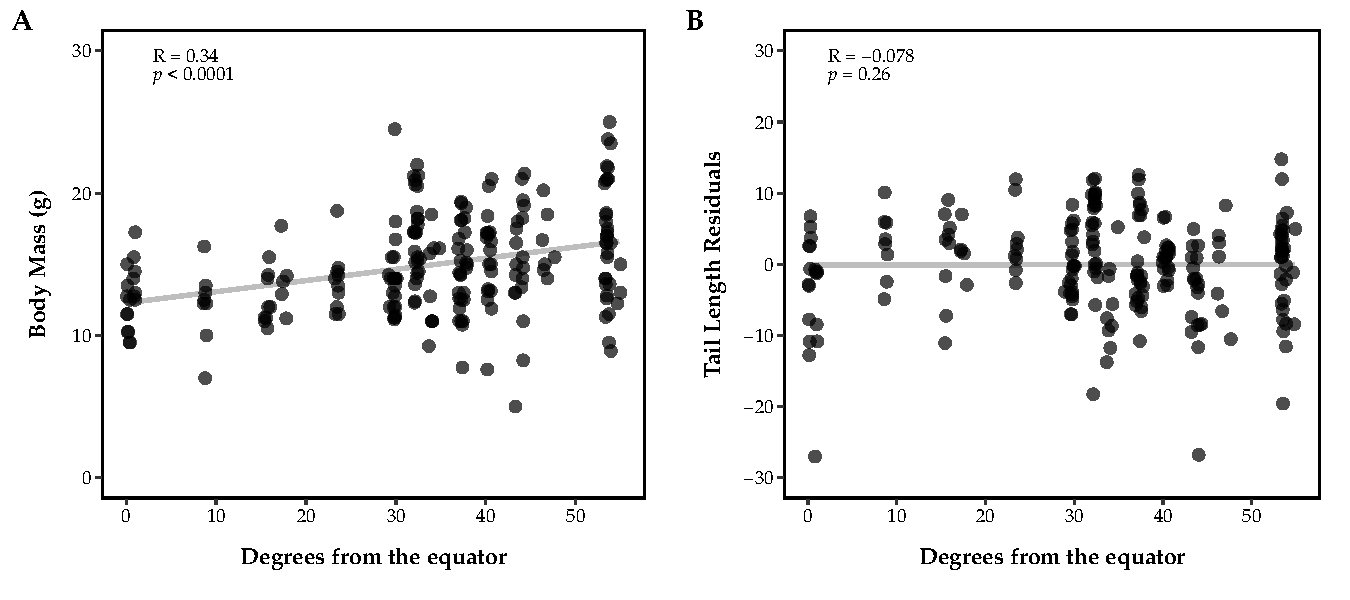
\includegraphics{../figures/Nachman_transects.pdf}

\textbf{Figure 1. The relationship between body weight, tail length, and
absolute latitude in North and South American house mice.} Significant
coorelation between body mass (A) and latitude, but not tail length (B)
and latitude in wild-caught house mice. Tail length residuals were
calculated by regressing tail length from body mass. Both plots include
males and females, with individuals represented as individual point.
Results from Spearman correlations are presented in each plot. Sample
sizes: (A) n = 215; (B) n = 212.

``Body mass in wild mice is linearly correlated with latitude (female: n
= xxx, rho = xxxx, p = xxxx''

\newpage

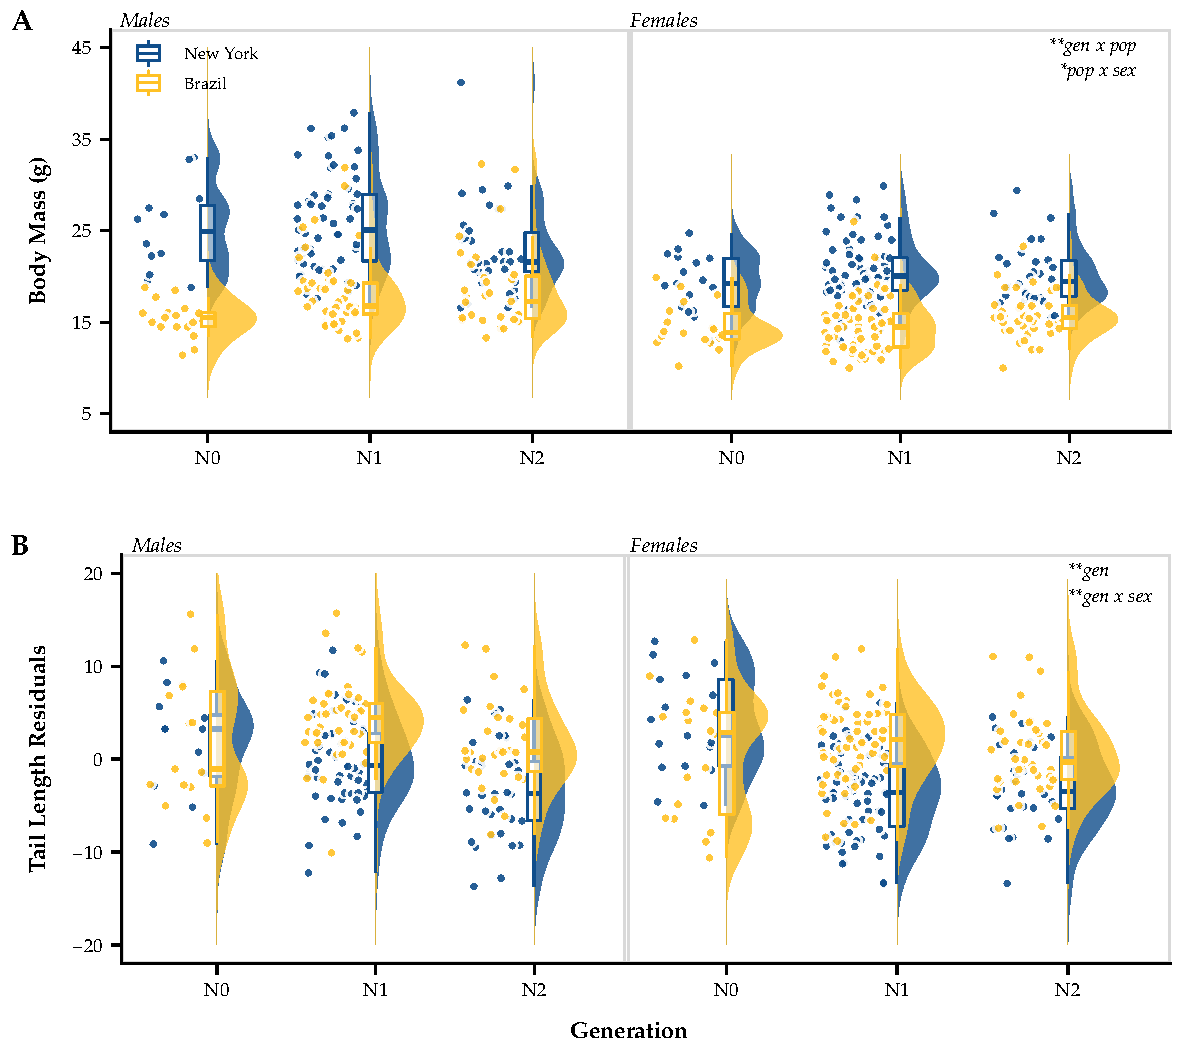
\includegraphics{../figures/generation_phenotypes.pdf}

\textbf{Figure 2. Body mass and tail length differences between
populations and across generations in a common lab environment.} ``Body
mass differences among populations persist over two generations in
lab''" (A), indicating a genetic basis. No clear differences in tail
length (B) are seen between populations, suggesting the inherent
``plastic''/``noisy'' nature of tail length. Tail length residuals were
calculated by regressing tail length from body mass. Population-level
data are depticted as boxplots overlayed on density plots, with boxplot
vertical lines denoting 1.5x the inerquartile range. Individuals are
represented as individual points. Results from linear mixed models are
presented in each plot. Only signifiant interactions are depicted in
(A). Sample sizes: (A) n = 438; (B) n = 427. *\emph{P}\textless{}0.05,
**\emph{*P} \textless{}0.01.

\newpage

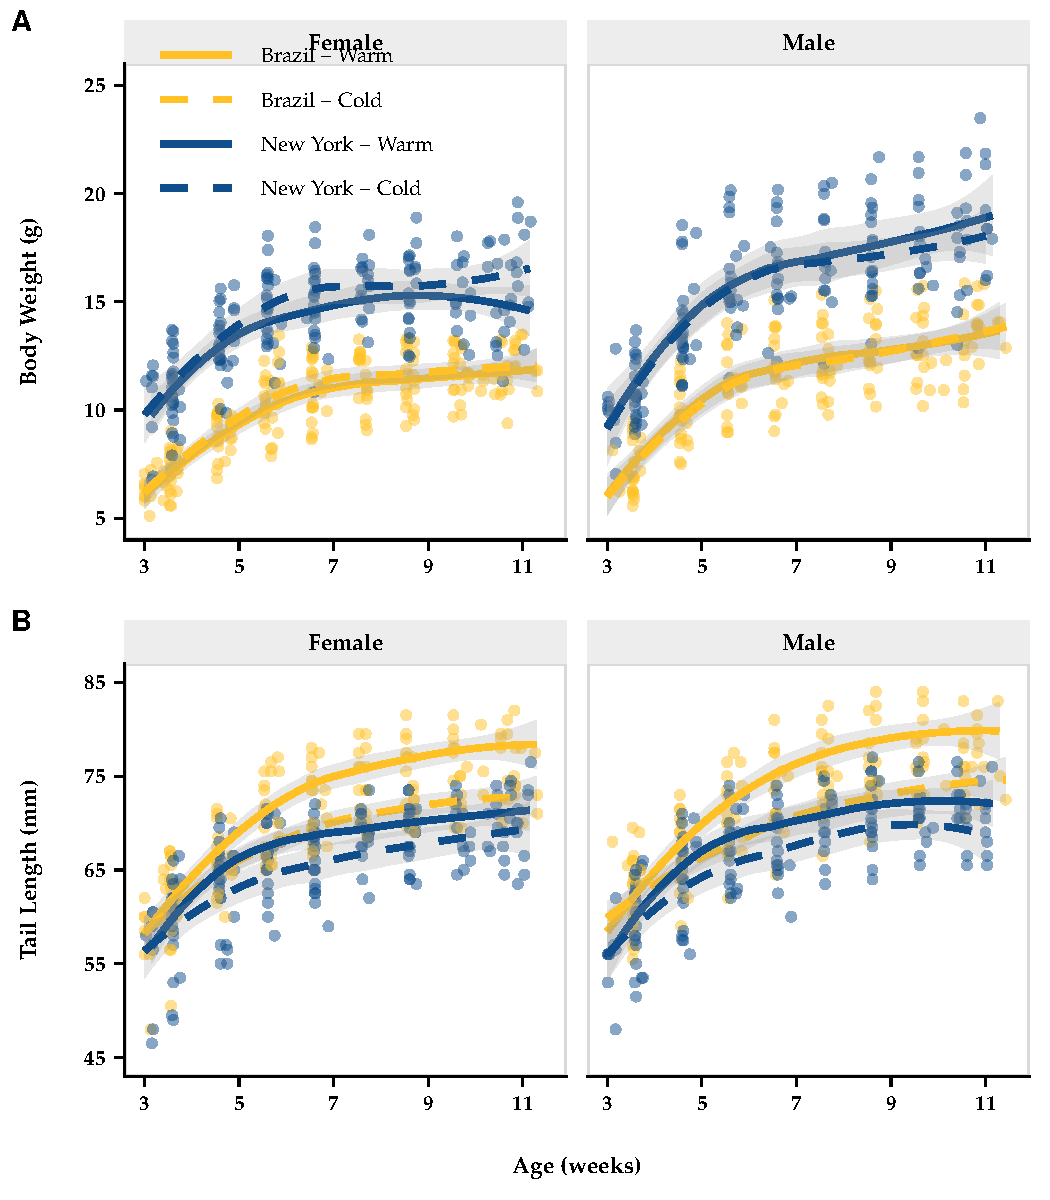
\includegraphics{../figures/weekly_phenotypes.pdf}

\textbf{Figure 3. Body mass and tail length growth trajectories across
environments.} Cold temperatures have very little influence on overall
body mass in New York and Brazil house mice (A). Tail length is highly
influenced by cold temperatures, with cold-housed mice growing shorter
tails compared to warm-housed mice (B). Both New York and Brazil house
mice show plasticity in tail length across development. Individuals are
represented as individual points (n = 80), with population means
depicted as smoothed regression fits, with standard error shading.

\newpage

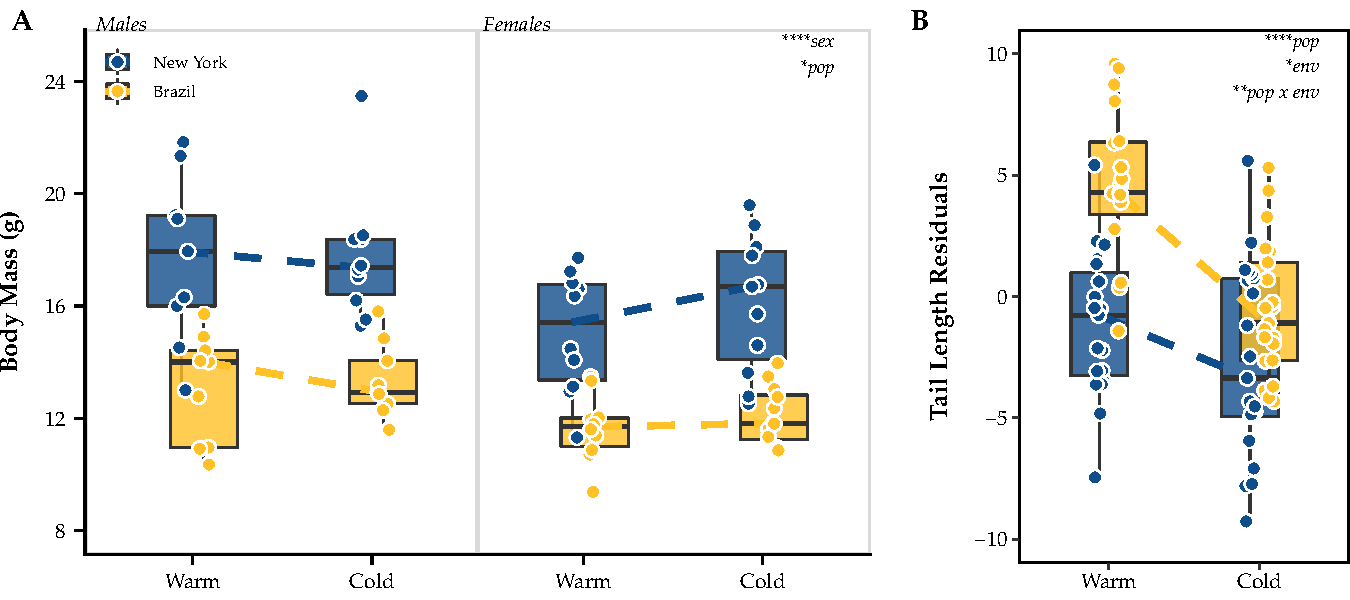
\includegraphics{../figures/RXNs.pdf}

\textbf{Figure 4. Evolved and plastic phenotypic variation among New
York and Brazil house mice.} Very little plasticity in body mass in New
York and Brazil house mice (A). Tail length is highly plastic in both
populations, with tails growing shorter in the cold (B). Brazil house
mice show adaptive plasticity in tail length. Tail length residuals were
calculated by regressing tail length from body mass. Vertical lines on
boxplots denote 1.5x the interquartile range. Individuals are
represented as individual points (n = 80). Results from linear mixed
models are presented in each plot, with the following significance
levels: *\emph{P}\textless{}0.05, **\emph{P} \textless{}0.01,
***\emph{P} \textless{}0.001, ****\emph{P} \textless{}0.0001

\newpage

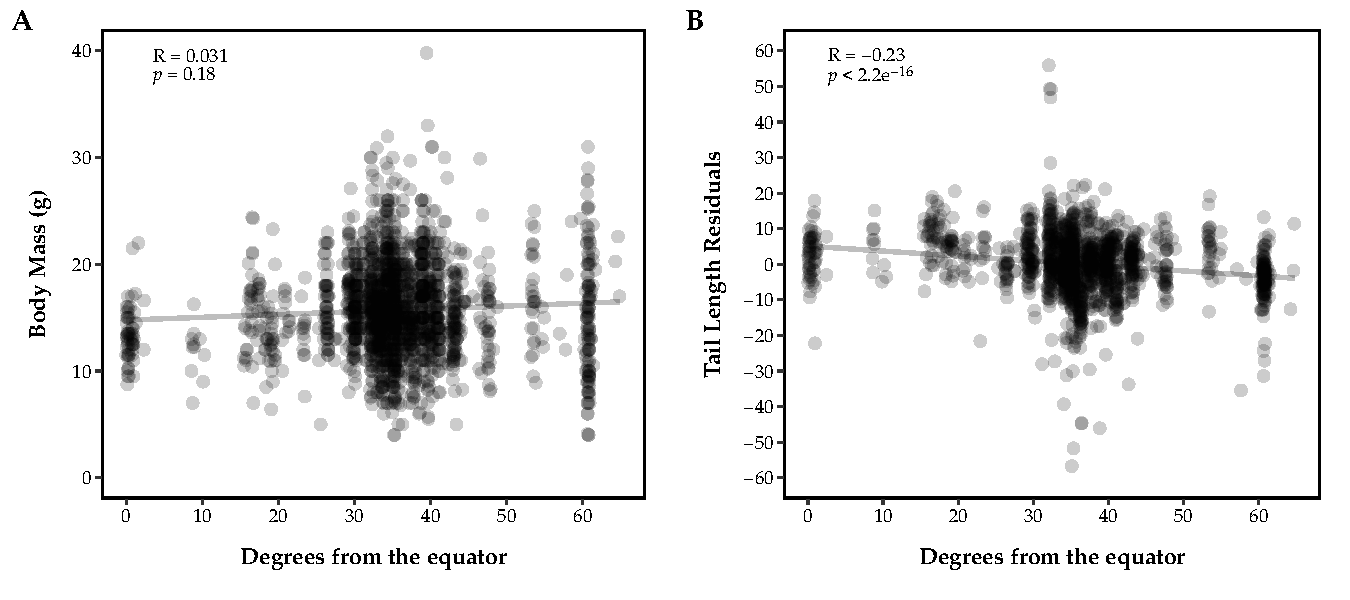
\includegraphics{../figures/VertNet_metadata.pdf}

\textbf{Figure S1. Bergmann's rule and Allen's rule using VertNet
metadata.}

\newpage

\hypertarget{acknowledgements}{%
\subsection{Acknowledgements}\label{acknowledgements}}

\newpage

\hypertarget{references}{%
\subsection{References}\label{references}}

\hypertarget{refs}{}
\leavevmode\hypertarget{ref-Allen1877}{}%
Allen, J. A. 1877. The influence of physical conditions in the genesis
of species. Radical review 1:108--140.

\leavevmode\hypertarget{ref-Barnett1984}{}%
Barnett, S., and R. Dickson. 1984. Changes among wild house mice (mus
musculus) bred for ten generations in a cold environment, and their
evolutionary implications. Journal of Zoology 203:163--180.

\leavevmode\hypertarget{ref-Bergmann1847}{}%
Bergmann, C. 1847. Über die verhältnisse der wärmeökonomie der thiere zu
ihrer grösse. Gottinger Studien 3:595--708.

\leavevmode\hypertarget{ref-Endler1977}{}%
Endler, J. A. 1977. Geographic variation, speciation, and clines.
Princeton University Press.

\leavevmode\hypertarget{ref-Harpak2021}{}%
Harpak, A., and M. Przeworski. 2021. The evolution of group differences
in changing environments. PLoS Biology 19:e3001072.

\leavevmode\hypertarget{ref-Huxley1938}{}%
Huxley, J. 1938. Clines: An auxiliary taxonomic principle. Nature
142:219--220.

\leavevmode\hypertarget{ref-James1983}{}%
James, F. C. 1983. Environmental component of morphological
differentiation in birds. Science 221:184--186.

\leavevmode\hypertarget{ref-Lynch1992}{}%
Lynch, C. B. 1992. Clinal variation in cold adaptation in mus
domesticus: Verification of predictions from laboratory populations. The
American Naturalist 139:1219--1236.

\leavevmode\hypertarget{ref-Phifer2018}{}%
Phifer-Rixey, M., K. Bi, K. G. Ferris, M. J. Sheehan, D. Lin, K. L.
Mack, S. M. Keeble, et al. 2018. The genomic basis of environmental
adaptation in house mice. PLoS Genetics 14:e1007672.

\leavevmode\hypertarget{ref-Phifer2015}{}%
Phifer-Rixey, M., and M. W. Nachman. 2015. The natural history of model
organisms: Insights into mammalian biology from the wild house mouse mus
musculus. Elife 4:e05959.

\leavevmode\hypertarget{ref-Suzuki2019a}{}%
Suzuki, T. A., F. M. Martins, and M. W. Nachman. 2019\emph{a}.
Altitudinal variation of the gut microbiota in wild house mice.
Molecular ecology 28:2378--2390.

\leavevmode\hypertarget{ref-Suzuki2020}{}%
Suzuki, T. A., F. M. Martins, M. Phifer-Rixey, and M. W. Nachman. 2020.
The gut microbiota and bergmann's rule in wild house mice. Molecular
Ecology 29:2300--2311.

\leavevmode\hypertarget{ref-Suzuki2019b}{}%
Suzuki, T. A., M. Phifer-Rixey, K. L. Mack, M. J. Sheehan, D. Lin, K.
Bi, and M. W. Nachman. 2019\emph{b}. Host genetic determinants of the
gut microbiota of wild mice. Molecular ecology 28:3197--3207.

\end{document}
